\chapter{The Challenge to Succeed (Part 1)}

These notes follow a Jim Rohn seminar talk, not a formal institutional course, and they preserve the reordered \emph{How You Got Successful?} sequence curated by LazyingArt LLC from Jim Rohn originals. The lecture is practical rather than technical, but it has a clear inner architecture. First, time is placed above money. Next, unequal compensation under equal outward conditions is traced to value rather than duration. Then the economic argument is widened into a philosophical one: what changes a life is not mainly what happens, but what we do. Finally, the whole discussion is reorganized by the seasonal model of life and business.

\section{Opening Contract: Time, Money, and the Right to Teach}

Rohn begins by converting attendance into an obligation on both sides. The audience has not merely bought a ticket; it has spent money, arranged dinner, transportation, and child care, and more importantly it has spent an evening, which he treats as a measurable piece of life. The opening law of the seminar is therefore not financial but evaluative:
\begin{equation}
T > M,
\end{equation}
where \(T\) denotes time and \(M\) money.

This relation is not presented as formal economics. It is the lecture's first working inequality. One can recover money, but one cannot recover the evening once spent. That is why the session is immediately described as work. We are told to take notes, to treat ideas as material to be captured, and not to confuse the seminar with entertainment. Even the light jokes at the beginning serve this larger point: the room is being made ready for concentration.

The autobiographical warrant then enters. Rohn presents himself first as a man who grew up in Idaho farm country, came from practical people, and knew the look of ordinary economic life. His parents remain examples of energy and practical intelligence; they are still busy, still developing land, and even appear in a concrete investment anecdote, buying gold at \(125\) and cashing out at \(680\). But the lecture is not moving toward inherited ease. It is moving toward crisis.

By age twenty-five he has already made promises larger than his results. He has married, he has promised wealth and travel, and the promised future is not arriving. The paycheck he names, \(57\) dollars, is not there for nostalgia. It is there to mark the mismatch between ambition and performance. The recurring phrase ``someday honey'' becomes a miniature model of deferred life: someday better furniture, someday a car, someday the promised world. What the lecture refuses is precisely this indefinite postponement.

At that point he does not yet know what to do. He considers going back to school, but that is not yet the answer. The decisive turn comes with Earl Shoaff, who enters the lecture not merely as an employer but as a source of philosophy. Rohn says explicitly that the best thing Shoaff gave him was not a job but a way of thinking. This is essential for the rest of the seminar. The speaker is claiming authority, but it is borrowed authority first, then tested, then passed on.

\section{From Shoaff to the Seminar Table of Contents}

Once Shoaff has entered the story, two linked themes appear: disciplined note-taking and transmissible philosophy. Shoaff teaches him to write things down, not to make the mind a filing cabinet, and to rely on repetition. Ideas repeated often enough, Rohn says, eventually show up in the bank account, the personality, the language, the dress, and the lifestyle. The sequence matters: the inner is not separated from the outer, but it appears first.

Years later, going through journals in Beverly Hills, Rohn decides to share those notes publicly. The first seminar is bad enough, he says, that had he not been the speaker he would have gone home. This is another important structural feature of the lecture. The public teacher is not introduced as naturally gifted; he is introduced as someone who struggled through repeated attempts until the material became speakable. The notes, then, are not private relics. They are the seed of the seminar form itself.

Only after that autobiography does he stop and give the audience a formal table of contents. The board is used here not as a place of derivation, but as a vertical outline of the evening.

\begin{figure}[t]
\centering

\includegraphics[width=0.82\linewidth]{lecture_18_figure_03.png}
\caption{Chalkboard outline of the seminar's major subjects. The upper line is partly obscured, but the spoken sequence immediately confirms the five-item outline.}
\end{figure}

The five subjects, in lecture order, are:
\begin{itemize}
\item Personal Development
\item Basic Laws
\item Goals
\item Diseases of Attitude
\item The Day That Turns Your Life Around
\end{itemize}

The screenshot preserves the board's vertical organization, and the transcript confirms the lines that are partly hidden by the speaker's body. A clean reconstruction is useful, but it should remain list-like rather than pretending to be a formal flowchart.

\begin{figure}[t]
\centering
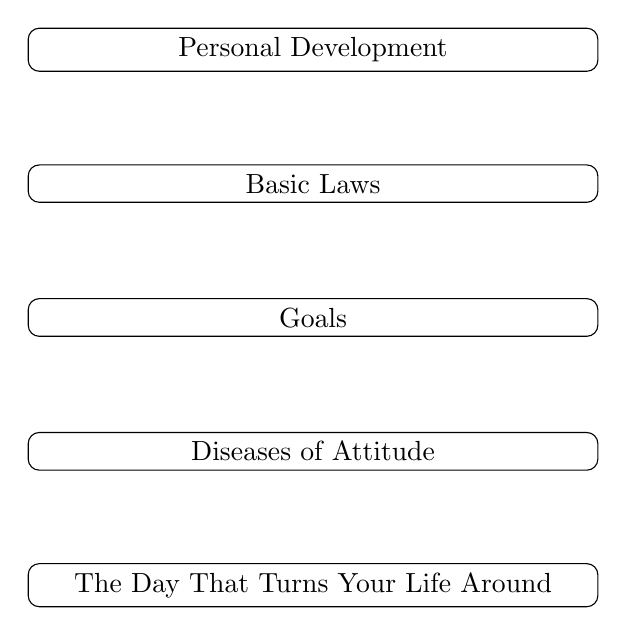
\begin{tikzpicture}
\node[draw, rounded corners, align=center, text width=7cm] at (0,0) {Personal Development};
\node[draw, rounded corners, align=center, text width=7cm] at (0,-1.7) {Basic Laws};
\node[draw, rounded corners, align=center, text width=7cm] at (0,-3.4) {Goals};
\node[draw, rounded corners, align=center, text width=7cm] at (0,-5.1) {Diseases of Attitude};
\node[draw, rounded corners, align=center, text width=7cm] at (0,-6.8) {The Day That Turns Your Life Around};
\end{tikzpicture}
\caption{Transcript-confirmed reconstruction of the board outline.}
\end{figure}

\subsection{Question \& Answer}

\paragraph{Question.} Why does the seminar begin with personal development rather than with goals, laws, or tactics?

\paragraph{Answer.} Because in this lecture the order is causal. The person comes before the techniques. If we do not begin with the one who acts, then later discussions of goals, attitude, and life-changing days lose their foundation. Rohn says this bluntly: if we do not start there, nothing much is going to happen.

\section{Personal Development as the Upstream Variable}

The lecture's first major doctrinal claim is that one can have more because one can become more. This is presented not as a slogan of optimism but as the rule that governs the rest of the evening:
\begin{equation}
\text{You can have more than you've got because you can become more than you are.}
\end{equation}
Its companion statement is equally sharp:
\begin{equation}
\text{Unless you change how you are, you will always have what you've got.}
\end{equation}

What gives these lines force is the next step. Rohn does not leave personal development in the air. He ties it to a practical law about income:
\begin{equation}
\text{Income does not far exceed personal development.}
\end{equation}
Sometimes income takes what he calls a lucky jump, but unless the person grows to match it, the gain recedes. The point is illustrated by the million-dollar example: if someone hands us a million dollars, we had better become a millionaire quickly, or the money will disappear. This is not a theorem about markets. It is the lecture's way of saying that gains which outrun character or skill are unstable.

A second law follows:
\begin{equation}
\text{Success is something you attract, not something you pursue.}
\end{equation}
Success is said to be looking for a good place to stay. That image explains why the lecture returns insistently to self-work. We are not told merely to run faster toward outcomes. We are told to become the kind of place where outcomes can remain.

This is why the seminar asks a particular question about employment. The important question on the job is not ``What am I getting?'' but ``What am I becoming?'' That reformulation is central. The lecture is not anti-income; it is against taking income as the first diagnostic. It is also why happiness is relocated from possession to formation: not what one gets, but what one becomes.

\begin{remark}
In these notes, ``personal development'' should be read as the lecture's upstream variable. It is not a vague mood. It is the practical condition that constrains retained income, durable success, and the quality of action.
\end{remark}

\section{Theme of the Seminar and the Compensation Puzzle}

After the table of contents and the first doctrine, the lecture pauses for its clearest visual maxim. The theme is written on the chalkboard in large cursive and treated as something to be carried into daily life.

\begin{figure}[t]
\centering

\includegraphics[width=0.82\linewidth]{lecture_18_figure_04.png}
\caption{The seminar theme written on the board.}
\end{figure}

The words are simple and presented with deliberate emphasis:
\begin{equation}
\text{The major key to your better future is you.}
\end{equation}
Rohn asks the audience to underline two words: \emph{major} and \emph{you}. The seminar theme is not that circumstances do not matter. It is that the largest controllable term in the equation of a better future is the person who acts.

From that maxim he moves immediately to the lecture's most compact practical puzzle. How can two people, under apparently similar external conditions, wind up with unequal compensation? He makes the matching conditions explicit: same company, same products, same services, same traffic, same problems, same community, perhaps even the same schooling and the same age. Yet the monthly result differs:
\begin{align}
Y_1 &= 1000 \text{ per month},\\
Y_2 &= 2000 \text{ per month}.
\end{align}
The question is not what the difference in dollars is. The question is what explains the difference.

At first he entertains a false answer: perhaps some people do better because they have more time. But that possibility is ruled out almost at once. There is no extra time to be found. When the day ends, it ends for everyone. In the seminar's compressed language, the quantity of time is effectively fixed:
\begin{equation}
T_1 = T_2.
\end{equation}

\subsection{Question \& Answer}

\paragraph{Question.} If time is fixed, what explains different results?

\paragraph{Answer.} The lecture's answer is that time cannot be the missing term. Once the outward conditions and the time interval are held fixed, the only meaningful question is what else can vary. That is the point at which Rohn introduces the key word of the evening: value.

\section{Value, Self-Work, and the Change Principle}

The word ``value'' is the turning point of the chapter. It is introduced not as a technical economic category but as the term that solves the compensation puzzle.

\begin{definition}
In the lecture's language, value is the quality of contribution brought to the marketplace and rewarded there. It is not a formal production variable. It is the practical name for what distinguishes one worker's result from another's when time alone does not.
\end{definition}

The central statement is given in verbal form:
\begin{equation}
\text{Value makes the difference in results.}
\end{equation}
and then tightened into an elementary rule of compensation:
\begin{equation}
\text{You get paid for value, not the time.}
\end{equation}

\begin{proposition}
Within the compensation puzzle of the lecture, if time is held fixed and compensation differs, the lecture directs us to look first at value rather than at duration.
\end{proposition}

\begin{proof}
Rohn deliberately matches the outward conditions of work and then contrasts unequal monthly income. In compressed notation we may write
\begin{align}
T_1 &= T_2,\\
Y_1 &= 1000 \text{ per month},\\
Y_2 &= 2000 \text{ per month}.
\end{align}
If \(T_1=T_2\), then the difference \(Y_2-Y_1\) is not explained by an additional supply of hours. The lecture therefore introduces value as the missing explanatory term. As editorial shorthand, faithful to the spoken argument but not presented by Rohn as formal notation, we may summarize the move by
\begin{equation}
T=\text{const},\qquad V\uparrow \Rightarrow Y\uparrow.
\end{equation}
\end{proof}

This shorthand lets us state the worked example Rohn himself poses. Is it possible to become twice as valuable and make twice as much money in the same time? Is it possible to become three times as valuable and make three times as much money in the same time? In the lecture's compressed language:
\begin{align}
V_2 = 2V_1 &\Rightarrow Y_2 \approx 2Y_1,\\
V_2 = 3V_1 &\Rightarrow Y_2 \approx 3Y_1.
\end{align}
The point is not a wage formula. The point is that the relevant variable is not more hours but more value.

\begin{remark}
These symbolic lines are note-taking aids. They should not be mistaken for a formal theory of labor markets. Rohn's claim is narrower and more practical: under matched outward conditions, value explains unequal compensation better than time does.
\end{remark}

The lecture then shifts from economics to cultivation of the self. An above-average income is tied to becoming an above-average person. The examples are concrete and modest: a better handshake, a better smile, more excitement, more interest in other people, more intensity to win. These are not decorations around the main doctrine. They are the first low-level examples of what ``more value'' looks like in ordinary conduct.

That is why Shoaff's instruction becomes the seminar's philosophical center:
\begin{equation}
\text{Work harder on yourself than you do on your job.}
\end{equation}

\begin{figure}[t]
\centering
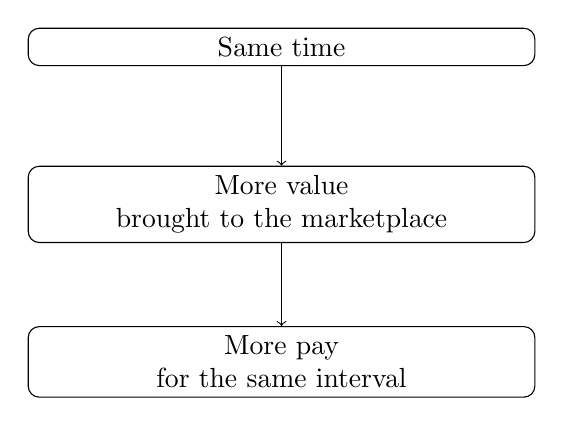
\begin{tikzpicture}
\node[draw, rounded corners, align=center, text width=6.2cm] (t) at (0,0) {Same time};
\node[draw, rounded corners, align=center, text width=6.2cm] (v) at (0,-2.0) {More value\\brought to the marketplace};
\node[draw, rounded corners, align=center, text width=6.2cm] (y) at (0,-4.0) {More pay\\for the same interval};
\draw[->] (t) -- (v);
\draw[->] (v) -- (y);
\end{tikzpicture}
\caption{Pocket-scale schematic of the lecture's compensation argument.}
\end{figure}

Once that instruction is stated, Rohn retrospectively understands why he was broke. He was a hard worker on the job, but not a hard worker on himself. The gap between labor and progress is therefore explained not by lack of effort in general, but by effort applied in the wrong direction.

\subsection{Question \& Answer}

\paragraph{Question.} If the world does not change, how can our life change?

\paragraph{Answer.} The lecture's answer is severe and simple:
\begin{equation}
\text{For things to change for you, you have to change.}
\end{equation}
The external order is not promised to rearrange itself. Therefore the controllable term is the self. That answer is then restated in its most compact form:
\begin{equation}
\text{The only way it gets better for you is when you get better.}
\end{equation}

\section{Not What Happens, but What We Do}

After the value argument, the lecture widens the field. It is no longer only a question of compensation. It becomes a general philosophy of causation in human life. The bridge to this larger claim is the destruction of excuses.

Rohn rehearses his old blame list with comic fullness: government, taxes, prices, weather, traffic, the car, manufacturers, company policy, the training program, negative relatives, cynical neighbors, the economy, the community. The list matters because it dramatizes a common habit of mind. We explain ourselves outward.

Shoaff's correction is then decisive. After hearing the list, he says: the big problem with your list is that you are not on it. That line is the hinge of the entire section. The list is torn up, and a fresh sheet is imagined with one word on it: \emph{Me}. The lecture is now ready to state its broadest law:
\begin{equation}
\text{It is not what happens; it is what you do.}
\end{equation}
The accompanying clarification is equally important:
\begin{equation}
\text{What happens is about the same; what people do is what is different.}
\end{equation}

This is why the lecture can absorb Murphy's laws without collapsing into fatalism. Yes, anything can happen. Everything can go wrong. Losses come. Money disappears. Disappointments arrive. But these are not special gifts reserved for one class of people. The point is not that events are mild. The point is that events are shared more widely than we like to think, and that reaction remains the decisive differentiator.

The rainstorm example makes the structure concrete:
\begin{enumerate}
\item One man sees the storm and stays home. For him, bad weather is a sufficient excuse to suspend effort.
\item Another man sees the same storm and reads it as opportunity. More people will be at home, and fewer salesmen will be out.
\end{enumerate}
The event is the same. The action differs. Therefore the result differs. This is the lecture's causal spine in miniature.

There is also a moral sharpening here. Once happenings are no longer treated as unique injuries, disappointment can no longer serve as a special exemption. ``Everybody has them,'' he says. The issue is not exemption but response.

\section{The Seasonal Model and the Four Major Lessons}

The final movement of the chapter reorganizes the whole lecture in a more memorable form. Rohn gives two phrases before giving four lessons:
\begin{equation}
\text{Life and business are like the changing seasons.}
\end{equation}
\begin{equation}
\text{You cannot change the seasons, but you can change yourself.}
\end{equation}

The first phrase describes the structure of external life. The second identifies the variable still under our control. This is the mature version of the earlier compensation argument. The same logic now governs the whole of life.

\begin{figure}[t]
\centering
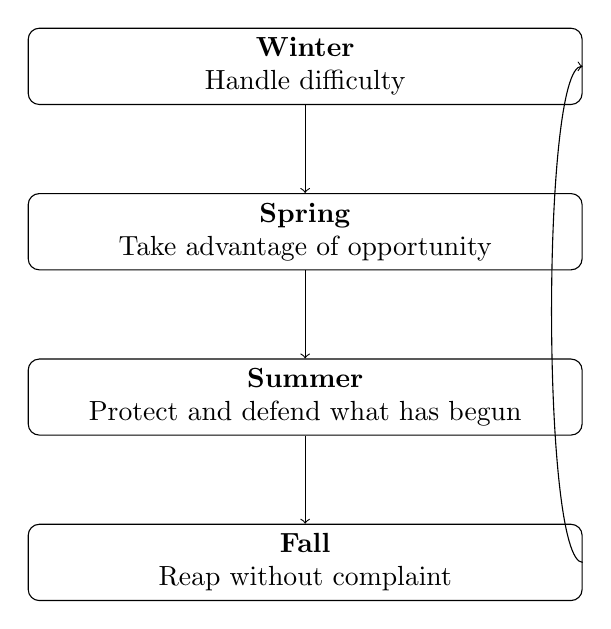
\begin{tikzpicture}
\node[draw, rounded corners, align=center, text width=6.8cm] (w) at (0,0) {\textbf{Winter}\\Handle difficulty};
\node[draw, rounded corners, align=center, text width=6.8cm] (sp) at (0,-2.1) {\textbf{Spring}\\Take advantage of opportunity};
\node[draw, rounded corners, align=center, text width=6.8cm] (su) at (0,-4.2) {\textbf{Summer}\\Protect and defend what has begun};
\node[draw, rounded corners, align=center, text width=6.8cm] (f) at (0,-6.3) {\textbf{Fall}\\Reap without complaint};
\draw[->] (w) -- (sp);
\draw[->] (sp) -- (su);
\draw[->] (su) -- (f);
\draw[->] (f.east) .. controls (3.0,-6.3) and (3.0,0.0) .. (w.east);
\end{tikzpicture}
\caption{A compact reconstruction of the lecture's seasonal cycle.}
\end{figure}

In note form, the cycle may be compressed as
\begin{equation}
\text{Winter} \to \text{Spring} \to \text{Summer} \to \text{Fall} \to \text{Winter}.
\end{equation}
Again, this is not a dynamical theory. It is a structural model for recurring conditions.

The four major lessons then unfold in transcript order.

\begin{enumerate}
\item \textbf{Learn how to handle the winters.} Difficulty is inevitable. Nights follow days, recession follows progression, and winter follows fall. One cannot remove January by tearing it off the calendar. Therefore the lecture's advice is not to wish winter away but to become stronger, wiser, and better. The associated maxim is one of Shoaff's strongest:
\begin{equation}
\text{Do not wish it were easier; wish you were better.}
\end{equation}

\item \textbf{Learn how to take advantage of the spring.} Opportunity follows difficulty. But spring itself is not enough. One must use it. Rohn's concrete line is that one must become good at one of two things: planting in the spring or begging in the fall. Opportunity has to be acted on, and acted on quickly, because there are only so many springs.

\item \textbf{Learn how to protect your crops all summer.} Here the lecture introduces two compact laws:
\begin{equation}
\text{All good will be attacked.}
\end{equation}
\begin{equation}
\text{All values must be defended.}
\end{equation}
This is the summer doctrine. Every garden is invaded. Therefore every value requires maintenance: political, social, communal, family, marital, friendship, business. Summer is the season of vigilance.

\item \textbf{Learn how to reap in the fall without complaint.} Harvest is the season of responsibility. If we do well, we need not apologize. If we do poorly, we must not complain. In either case, adulthood is marked by accepting responsibility for what has happened.
\end{enumerate}

This last point is more severe than it first appears. The lecture is not asking merely for emotional toughness. It is asking us to move from explanation to ownership. That is why the section on excuses had to come before the section on harvest.

\subsection{Question \& Answer}

\paragraph{Question.} What can we do starting tomorrow that will make a difference?

\paragraph{Answer.} The lecture deliberately leaves this question alive rather than closing it with a formula. The first answer is negative: if nothing changes tomorrow, then the next five years will resemble the last five. The second answer is structural: one cannot stop winter, command spring, or prevent attack by wish alone. One can, however, change direction through action. The lecture's demand is therefore not for a mystical breakthrough but for an initiating act of change. Even a small real change alters the path; no change leaves the path intact.

\section{Summary}

Part 1 of this lecture proceeds by a surprisingly tight chain. An evening of life is more valuable than the money spent to attend. Because time is fixed, unequal compensation must be explained by value rather than by duration. Because value can be increased, one must work on oneself rather than merely on the job. Because the world does not rearrange itself on request, the person must change. Because happenings are widely shared, response is what differentiates lives. And because life and business move in seasons, wisdom consists not in abolishing winter but in learning how to move through the whole cycle with strength, initiative, defense, and responsibility.

The chapter therefore ends where the lecture wants it to end: not with closure, but with a demand. Starting tomorrow, what shall we do that makes a difference?